\section{Introduction}

\subsection{Motivation}

\begin{frame}{Matthias Kuhn}
	\begin{columns}[T] % contents are top vertically aligned
		\begin{column}[T]{5cm} % each column can also be its own environment
			\begin{itemize}
				\item QGIS Core Developer
				\item Co-Founder and CTO of OPENGIS.ch Ltd
				\item Skier and Mountaineer
			\end{itemize}
		\end{column}
		\begin{column}[T]{5cm} % alternative top-align that's better for graphics
			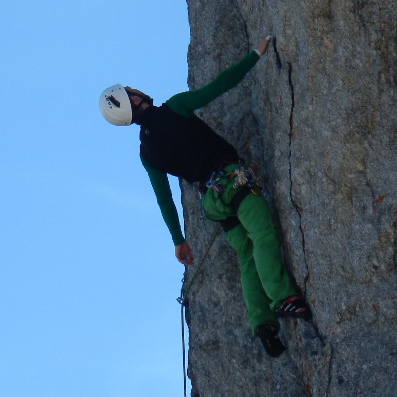
\includegraphics[height=3.5cm]{img/matthias.png}
		\end{column}
	\end{columns}
\end{frame}

\begin{frame}
\frametitle{Version 0.9 'Ganymede' (2007)}
	\begin{itemize}
		\item \textbf{Python bindings - This is the major focus of this release
			it is now possible to create plugins using python. It is also
			possible to create GIS enabled applications written in python 
			that use the QGIS libraries.}
		\item Removed automake build system - QGIS now needs CMake for compilation.
		\item Many new GRASS tools added (with thanks to http://faunalia.it/)
		\item Map Composer updates
		\item Crash fix for 2.5D shapefiles
		\item The QGIS libraries have been refactored and better organised.
		\item Improvements to the GeoReferencer
	\end{itemize}
\end{frame}

\begin{frame}
\frametitle{Plugin ecosystem}
	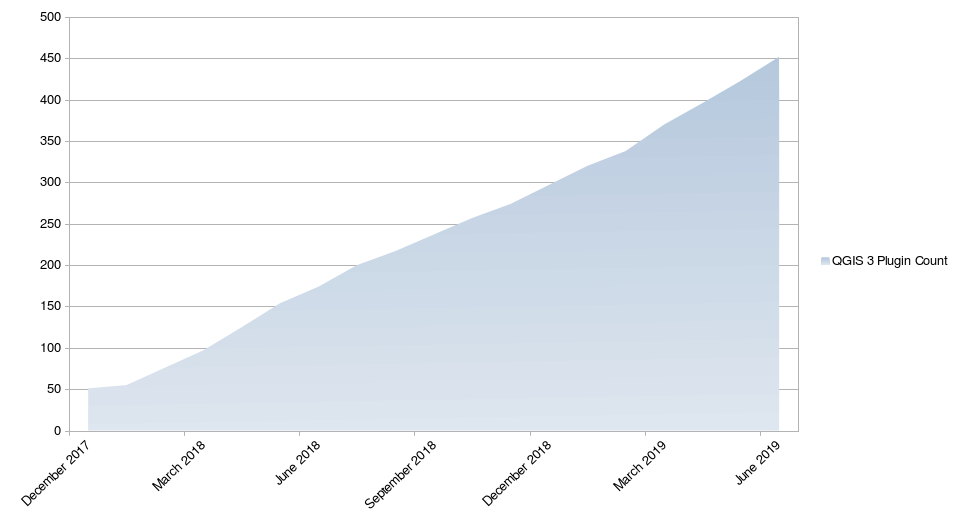
\includegraphics[width=0.9\textwidth]{img/qgis_plugin_count.png}

	(because every presentation needs a trend graph)
\end{frame}

\begin{frame}
\frametitle{Optimizing PyQGIS}

\begin{itemize}
	\item Various collections of "common pyqgis helper functions" have been written to "make things easier".
\end{itemize}

See: \url{http://osgeo-org.1560.x6.nabble.com/QGIS-Developer-Common-PyQGIS-functions-for-QGIS-3-td5395644.html}
\end{frame}

\begin{frame}
\frametitle{Common PyQGIS functions for QGIS 3}
\epigraph{``Wouldn't it be possible to provide such a collection of common pyqgis functions not only from private persons/projects but from the QGIS-project itself so users could add common functions?
I think the chances would be higher that such a "official" collection would be used in the long run and constantly extended."}{--- Thomas Baumann, QGIS Developer Mailing List}
\end{frame}

\begin{frame}
\frametitle{The goal}
\begin{description}
	\item [API first] Make flexible and easy to use APIs. Benefits Python and C++.
	\item [Pythonic] Implement ``Pythonic" constructs. Leverage modern Python language features.
\end{description}
\end{frame}